\documentclass[notes,xelatex,13pt]{beamer}
\usetheme{metropolis}
\usefonttheme{professionalfonts} % using non standard fonts for beamer
\usefonttheme{serif}
\usepackage{helvet}
\usepackage[english]{babel}
\usepackage{graphicx}
\usepackage{textpos}
\usepackage{pgfpages}

\setbeamertemplate{note page}{\pagecolor{yellow!5}\insertnote}\usepackage{palatino}
\setbeameroption{show notes on second screen}

\beamertemplatenavigationsymbolsempty

\usepackage{xkeyval}
\usepackage{todonotes}
\presetkeys{todonotes}{inline}{}

\title{Asynchronous single page applications without a line of HTML or
Javascript.}
\subtitle{Or why D is just awesome}
\author{Robert "burner" Schadek}
\date{May 5, 2016}
\institute{DConf}

\begin{document}
\maketitle

\begin{frame}
	\frametitle{Javascript and HTML are \textbf{awesome}}
	\begin{itemize}
		\item No types
		\item Variables may be undefined
		\item Repetition repetition repetition
		\item No templates
		\item No compile time function execution
			\pause
		\item No compile time
	\end{itemize}
	\note[item]{Very quickly go through the points and stop for dramatic pause}
\end{frame}


\begin{frame}[plain]
\begin{textblock*}{0cm}(-1cm,-4.2cm)
	
\includegraphics[width=1.0\paperwidth]{picardriker.jpg}
\end{textblock*}
	\note[item]{I know what you are thinking.}
	\note[item]{Walter, Andrei and the other screwed up letting me present
	here.}
\end{frame}

\begin{frame}
	\frametitle{Goals}	
	\begin{itemize}
		\item Retain type-information of data from DB to Client's Browser
			\pause
		\item Keeping things DRY	
			\pause
		\item Get things done
			\pause
	\end{itemize}
\end{frame}

\section{Vibe.d and Diet}
\begin{frame}
	\frametitle{Vibe.d and Diet}
	\todo{REST Interface generator}
	\todo{Web Client generator}
	\todo{Async sockets}
	\todo{Async mysql}
	\todo{Session (Redis)}
\end{frame}

\section{Typescript and AngularJS}
\begin{frame}
	\frametitle{Typescript and AngularJS}
\end{frame}

\section{Dataflow from the Frontend to the Database and back again}
\begin{frame}
	\frametitle{Dataflow from the Frontend to the Database and back again}
\end{frame}

\section{Testing and Debugging}
\begin{frame}
	\frametitle{Testing and Debugging}
	\note[item]{Of course we are perfect programmers and never make mistakes,
	\textbf{BUT}.}
\end{frame}

\section{Everything is wrong}
\begin{frame}
\begin{textblock*}{0cm}(-1cm,-4.2cm)
	
\includegraphics[width=1.0\paperwidth]{picarddday.jpg}
\end{textblock*}
\end{frame}

\begin{frame}
	\frametitle{Everything is wrong}
	\begin{itemize}
		\item all we solved was a tiny specific problem
		\item what about server to database
		\item what if we would use Dart instead of Typescript
		\item how do we communicate the overall architecture
		\item how do we keep the architecture in sync with the code
		\item how do we communicate with non-developer
		\item ...
		\pause
		\item {\huge How do we deal with change?}
	\end{itemize}
\end{frame}

\begin{frame}
	\frametitle{Everything is still wrong}
	\begin{itemize}
		\onslide<1->{\item Waterfall Model} \onslide<2->{\(\leftarrow\) no change ever}
		\onslide<7->{\item UML} \onslide<8->{\(\leftarrow\) just kill me
			already}

		\item[] { \onslide<1-8>{
\includegraphics[width=0.3\textwidth]{Stick1.png}}
				\only<9>{
\includegraphics[width=0.3\textwidth]{Stick.png}}
				\only<10>{
\includegraphics[width=0.3\textwidth]{Stick2.png}}
		}

		\onslide<5->{\item agile Methods} \onslide<6->{\(\leftarrow\) just
			hacking with fancy names}
		\onslide<3->{\item just Hacking} \onslide<4->{\(\leftarrow\) no plan
			to speak of, just change}
		
	\end{itemize}
	
\end{frame}

\begin{frame}
	\frametitle{What do we want}
	\begin{itemize}
		\item speak about the system at different levels of detail\\
		with different people
		\item quickly introduce people to the system
		\item keep data classes (Model) synchronized across
		\begin{itemize}
			\item Frontend
			\item Server
			\item Database
		\end{itemize}
		\item write only one model for everything, to keep stuff in sync
		\item have description line based, because git
		\item generate everything possible from the
	\end{itemize}
\end{frame}

\section{Introducing C4 Architecture}
\begin{frame}[plain]
\begin{textblock*}{0cm}(-1cm,-4.7cm)
	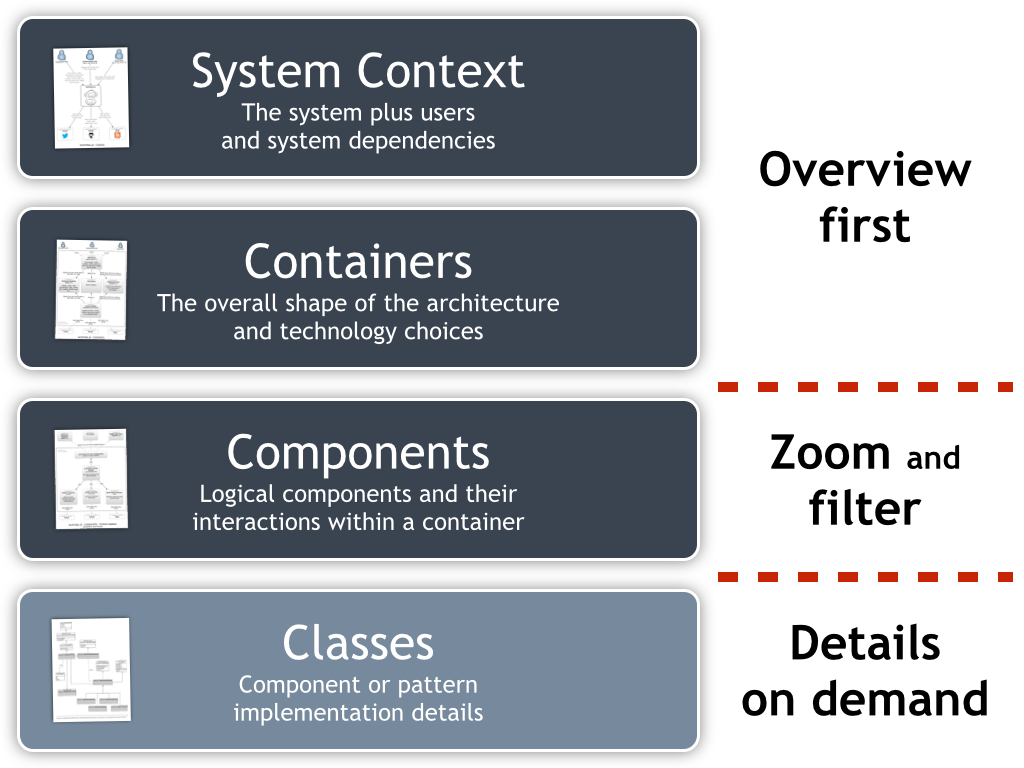
\includegraphics[width=1.0\paperwidth]{c4overview.png}
\end{textblock*}
\end{frame}
\begin{frame}[plain]
\begin{textblock*}{0cm}(-1cm,-4.7cm)
	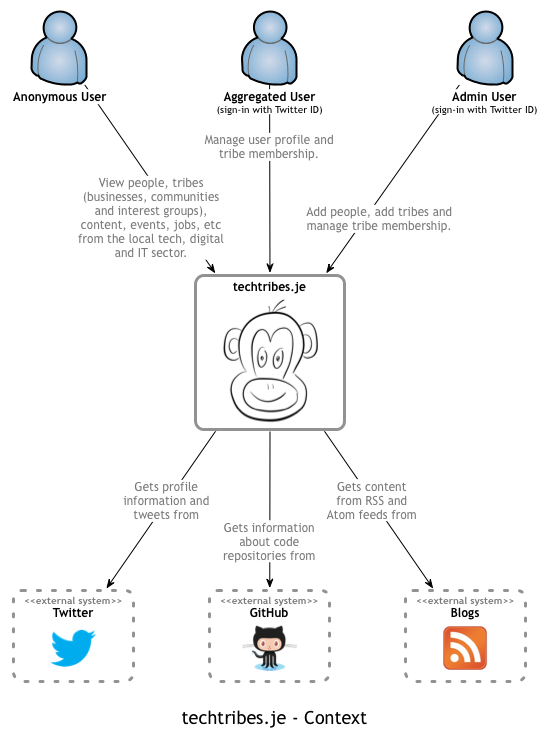
\includegraphics[width=1.0\paperwidth]{c4systemcontext.png}
\end{textblock*}
\end{frame}
\begin{frame}[plain]
\begin{textblock*}{0cm}(-1cm,-11.7cm)
	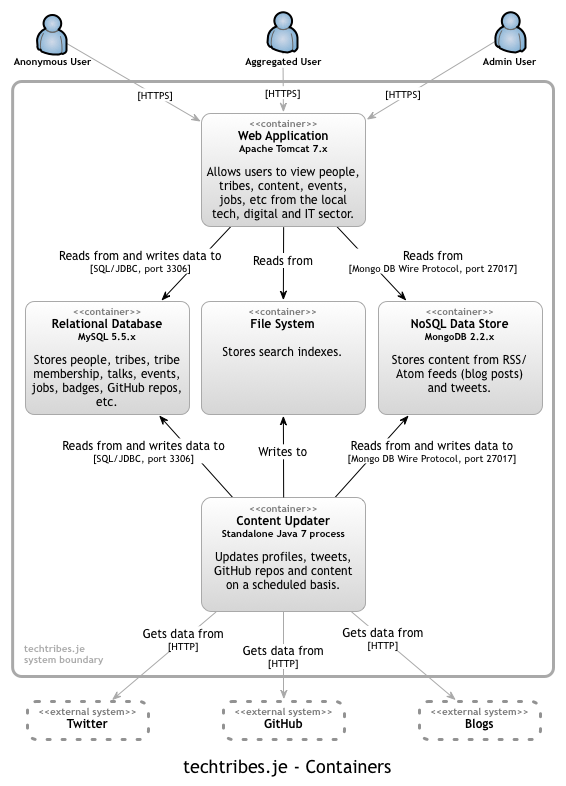
\includegraphics[width=1.0\paperwidth]{c4container.png}
\end{textblock*}
\end{frame}
\begin{frame}[plain]
\begin{textblock*}{0cm}(-1cm,-4.7cm)
	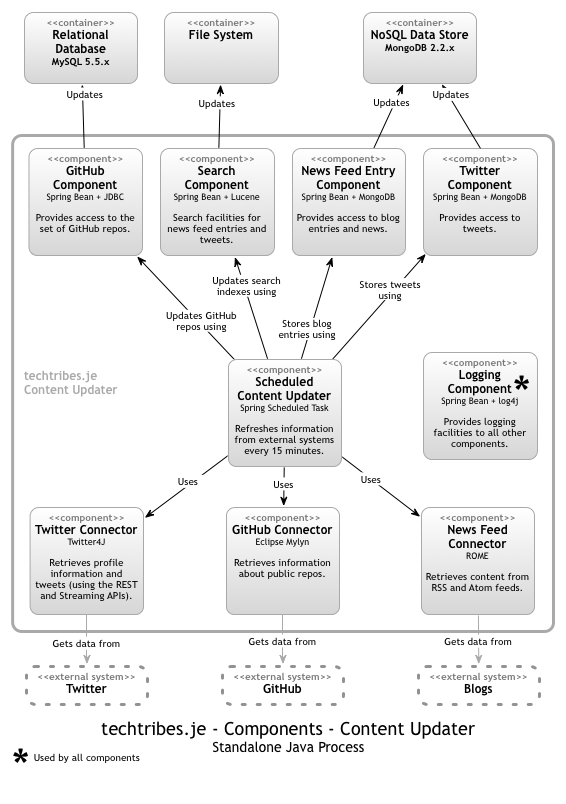
\includegraphics[width=1.0\paperwidth]{c4components.png}
\end{textblock*}
\end{frame}

\begin{frame}
	\frametitle{C4 Architecture \/ Structurizer}
	\begin{itemize}
		\item Awesome
		\item Java Library with classes to build this model
		\begin{itemize}
			\item its code, its fits into gilt
		\end{itemize}
		\item Structurizer even generates code  
		\item[] only Java spring and .net
	\end{itemize}
\end{frame}
\begin{frame}[plain]
\begin{textblock*}{0cm}(-1cm,-4.2cm)
	
\includegraphics[width=1.0\paperwidth]{picardwtf.jpg}
\end{textblock*}
\end{frame}

\section{Miscellaneous}
\begin{frame}
	\frametitle{Miscellaneous}
	\todo{GC Angst}
	\todo{Deployment}
	\todo{Performance Tuning}
	\todo{HTTPS}
\end{frame}

\begin{frame}[plain]
\begin{textblock*}{0cm}(-1cm,-4.2cm)
	
\includegraphics[width=1.0\paperwidth]{picardpuppy.png}
	\todo{http://gryphon-shifter.deviantart.com/art/Captain-Picard-and-Puppies-458352865}
\end{textblock*}
\end{frame}

\end{document}
